\subsubsection{背景}
在 VQE 中高精度模拟分子体系是一项同时消耗时间和内存的任务。不同规模氢链模拟所需的内存如表 \ref{tab:memory_h_chain} 所示。

\begin{table}[ht]
    \begin{tabular}{ccc}
        \toprule
        氢链 & 量子比特数 & Complex128 内存占用 \\
        \midrule
        $H_2$          & 4            & 0.256kB                \\
        $H_6$          & 12           & 64kB                   \\
        $H_{10}$       & 20           & 16MB                   \\
        $H_{14}$       & 28           & 4GB                    \\
        $H_{18}$       & 36           & 1TB                    \\
        \bottomrule
    \end{tabular}
    \caption{存储全振幅量子态所需的内存开销。}
    \label{tab:memory_h_chain}
\end{table}

基于 UCCSD（Unitary coupled-cluster with singles and doubles，单、双激发酉耦合簇）理论，ansatz 可描述为：
\begin{equation}
    |\Psi(\vec{\theta})\rangle = e^{(\hat{T}-\hat{T}^\dagger)}\ket{\psi_\text{HF}},
\end{equation}
其中 $\hat{T}$ 是耦合簇算符，$\ket{\psi_\text{HF}}$ 是 Hartree-Fock 态。耦合簇算符写作：
\begin{equation}
    \hat{T}=\sum_{p\notin\text{occ},q\in\text{occ}}\theta_q^p \hat{a}_p^\dagger \hat{a}_q + \sum_{pq\notin\text{occ},rs\in\text{occ}}\theta_{rs}^{pq}\hat{a}_p^\dagger \hat{a}_q^\dagger \hat{a}_r \hat{a}_s,
\end{equation}
在一阶 Trotter 分解下，ansatz 可分解为：
\begin{equation}
    |\Psi(\vec{\theta})\rangle\approx \prod_ie^{(\hat{T}_i-\hat{T}_i^\dagger)}\ket{\psi_\text{HF}}.
\end{equation}
以氢链 $H_6$ 为例，模拟该系统需要 12 个量子比特，其中包含 6 个电子，3 个自旋向上、3 个自旋向下。图 \ref{6_1_h6_a} 展示了 $H_6$ 的 Hartree-Fock 态，图 \ref{6_1_h6_b} 展示了在激发算符 $\hat{T}=\hat{a}_{11}^\dagger \hat{a}_{10}^\dagger \hat{a}_5 \hat{a}_4$ 作用下的自旋轨道。
\begin{figure}
    \centering
    \begin{subfigure}{0.3\textwidth}
        \centering
        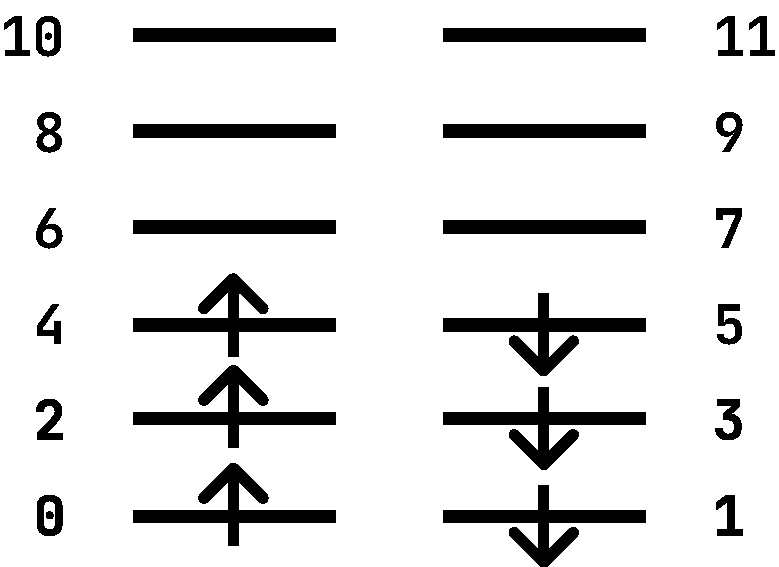
\includegraphics[width=\textwidth]{images/6_1_h6_a.pdf}
        \caption{$H_6$ 的 Hartree-Fock 态。}
        \label{6_1_h6_a}
    \end{subfigure}
    \begin{subfigure}{0.3\textwidth}
        \centering
        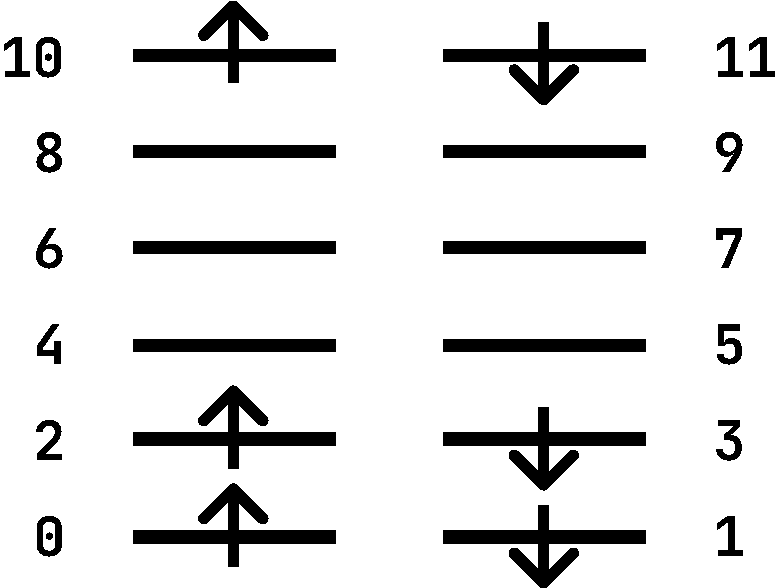
\includegraphics[width=0.9\textwidth]{images/6_1_h6_b.pdf}
        \caption{作用激发算符 $\hat{T}=\hat{a}_{11}^\dagger \hat{a}_{10}^\dagger \hat{a}_5 \hat{a}_4$ 后的自旋轨道。}
        \label{6_1_h6_b}
    \end{subfigure}
\end{figure}
\subsubsection{电子数和自旋守恒}
在 \QuPack\ 中，我们施加了总电子数和电子总自旋数在 ansatz 演化过程中保持不变的约束。该约束显著降低了需要模拟的 Hilbert 空间维度。假设量子比特数为 $n_q$、电子数为 $n_e$，全振幅态的维度为 $2^{n_q}$；而在施加电子数和自旋守恒约束后，维度变为：
\begin{equation}
    \binom{n_q/2}{n_e/2}^2=\left(\frac{(n_q/2)!}{(n_e/2)!(n_q/2-n_e/2)!}\right)^2.
\end{equation}
内存开销将从 1TB 降低到约 35GB。

除降低内存外，我们还优化了耦合簇算符的演化。对于给定的耦合簇算符 $\hat{V}(\theta)=e^{\theta(\hat{T}-\hat{T}^\dagger)}$，容易证明 $(\hat{T}-\hat{T}^\dagger)^3 = - (\hat{T}-\hat{T}^\dagger)$，且 $(\hat{T}-\hat{T}^\dagger)^4 = -(\hat{T}-\hat{T}^\dagger)^2$。经过 Taylor 展开可得：
\begin{equation}
    \hat{V}(\theta) = \mathbb{I} + ( 1-\cos\theta)(\hat{T}-\hat{T}^\dagger)^2 + \sin\theta (\hat{T}-\hat{T}^\dagger).
\end{equation}
在约化 Hilbert 空间中选取一个计算基 $\ket{i}$，使得 $\hat{T}\ket{i} = \ket{j}\neq0$，则有 $\hat{T}^\dagger\ket{i}=0$ 且 $\hat{T}^\dagger\ket{j}=\ket{i}$。耦合簇演化可简化为：
\begin{equation}
    e^{\theta(\hat{T}-\hat{T}^\dagger)}\begin{pmatrix}
        \ket{i} \\\ket{j}
    \end{pmatrix}=\begin{pmatrix}
        \cos\theta  & \sin\theta \\
        -\sin\theta & \cos\theta
    \end{pmatrix}\begin{pmatrix}
        \ket{i} \\\ket{j}
    \end{pmatrix}.
\end{equation}
对于 $e^{i\theta(\hat{T}+\hat{T}^\dagger)}$，则有
\begin{equation}
    e^{i\theta(\hat{T}+\hat{T}^\dagger)}\begin{pmatrix}
        \ket{i} \\\ket{j}
    \end{pmatrix}=\begin{pmatrix}
        \cos\theta   & i\sin\theta \\
        -i\sin\theta & \cos\theta
    \end{pmatrix}\begin{pmatrix}
        \ket{i} \\\ket{j}
    \end{pmatrix}.
\end{equation}

在该系统上执行变分量子算法时，需要计算 $\hat{V}(\theta)$ 的梯度，其形式为：
\begin{equation}
    \frac{\partial \hat{V}(\theta)}{\partial\theta}\begin{pmatrix}
        \ket{i} \\\ket{j}
    \end{pmatrix}=\begin{pmatrix}
        -\sin\theta & \cos\theta  \\
        -\cos\theta & -\sin\theta
    \end{pmatrix}\begin{pmatrix}
        \ket{i} \\\ket{j}
    \end{pmatrix}.
\end{equation}

下面的示例代码展示了如何构建耦合簇算符演化对应的量子线路。

\begin{lstlisting}
from qupack.vqe import ExpExciteGate
from mindquantum.algorithm.nisq import uccsd_singlet_generator
from mindquantum.core.circuit import Circuit

ucc_fermion_ops = uccsd_singlet_generator(6, 4)
circ = Circuit()
for term in ucc_fermion_ops:
    circ += ExpExciteGate(term)
\end{lstlisting}

为在 Hilbert 空间的子空间内高效模拟耦合簇算符，我们设计了一个名为 \code{ESConservation} 的专用模拟器。该模拟器与 \MindQuantum\ 中的模拟器共享相同 API，并擅长精确刻画这些算符的复杂动力学。
